\section{Паралелне улазно/излазне операције}

Паралелне улазно/излазне операције у MPI програму се обављају функцијама које су сличне стандардним \zn језичким" улазно/излазним функцијама и библиотекама. MPI има неколико додатних функција које побољшавају  учинак и портабилност програма. Основна карактеристика MPI је да може изразити паралелизам у овим операцијама. Секвенцијалне улазно/излазне операције паралелног програма приказане су на слици 2.1.

\begin{figure}[h!]
  \centering
      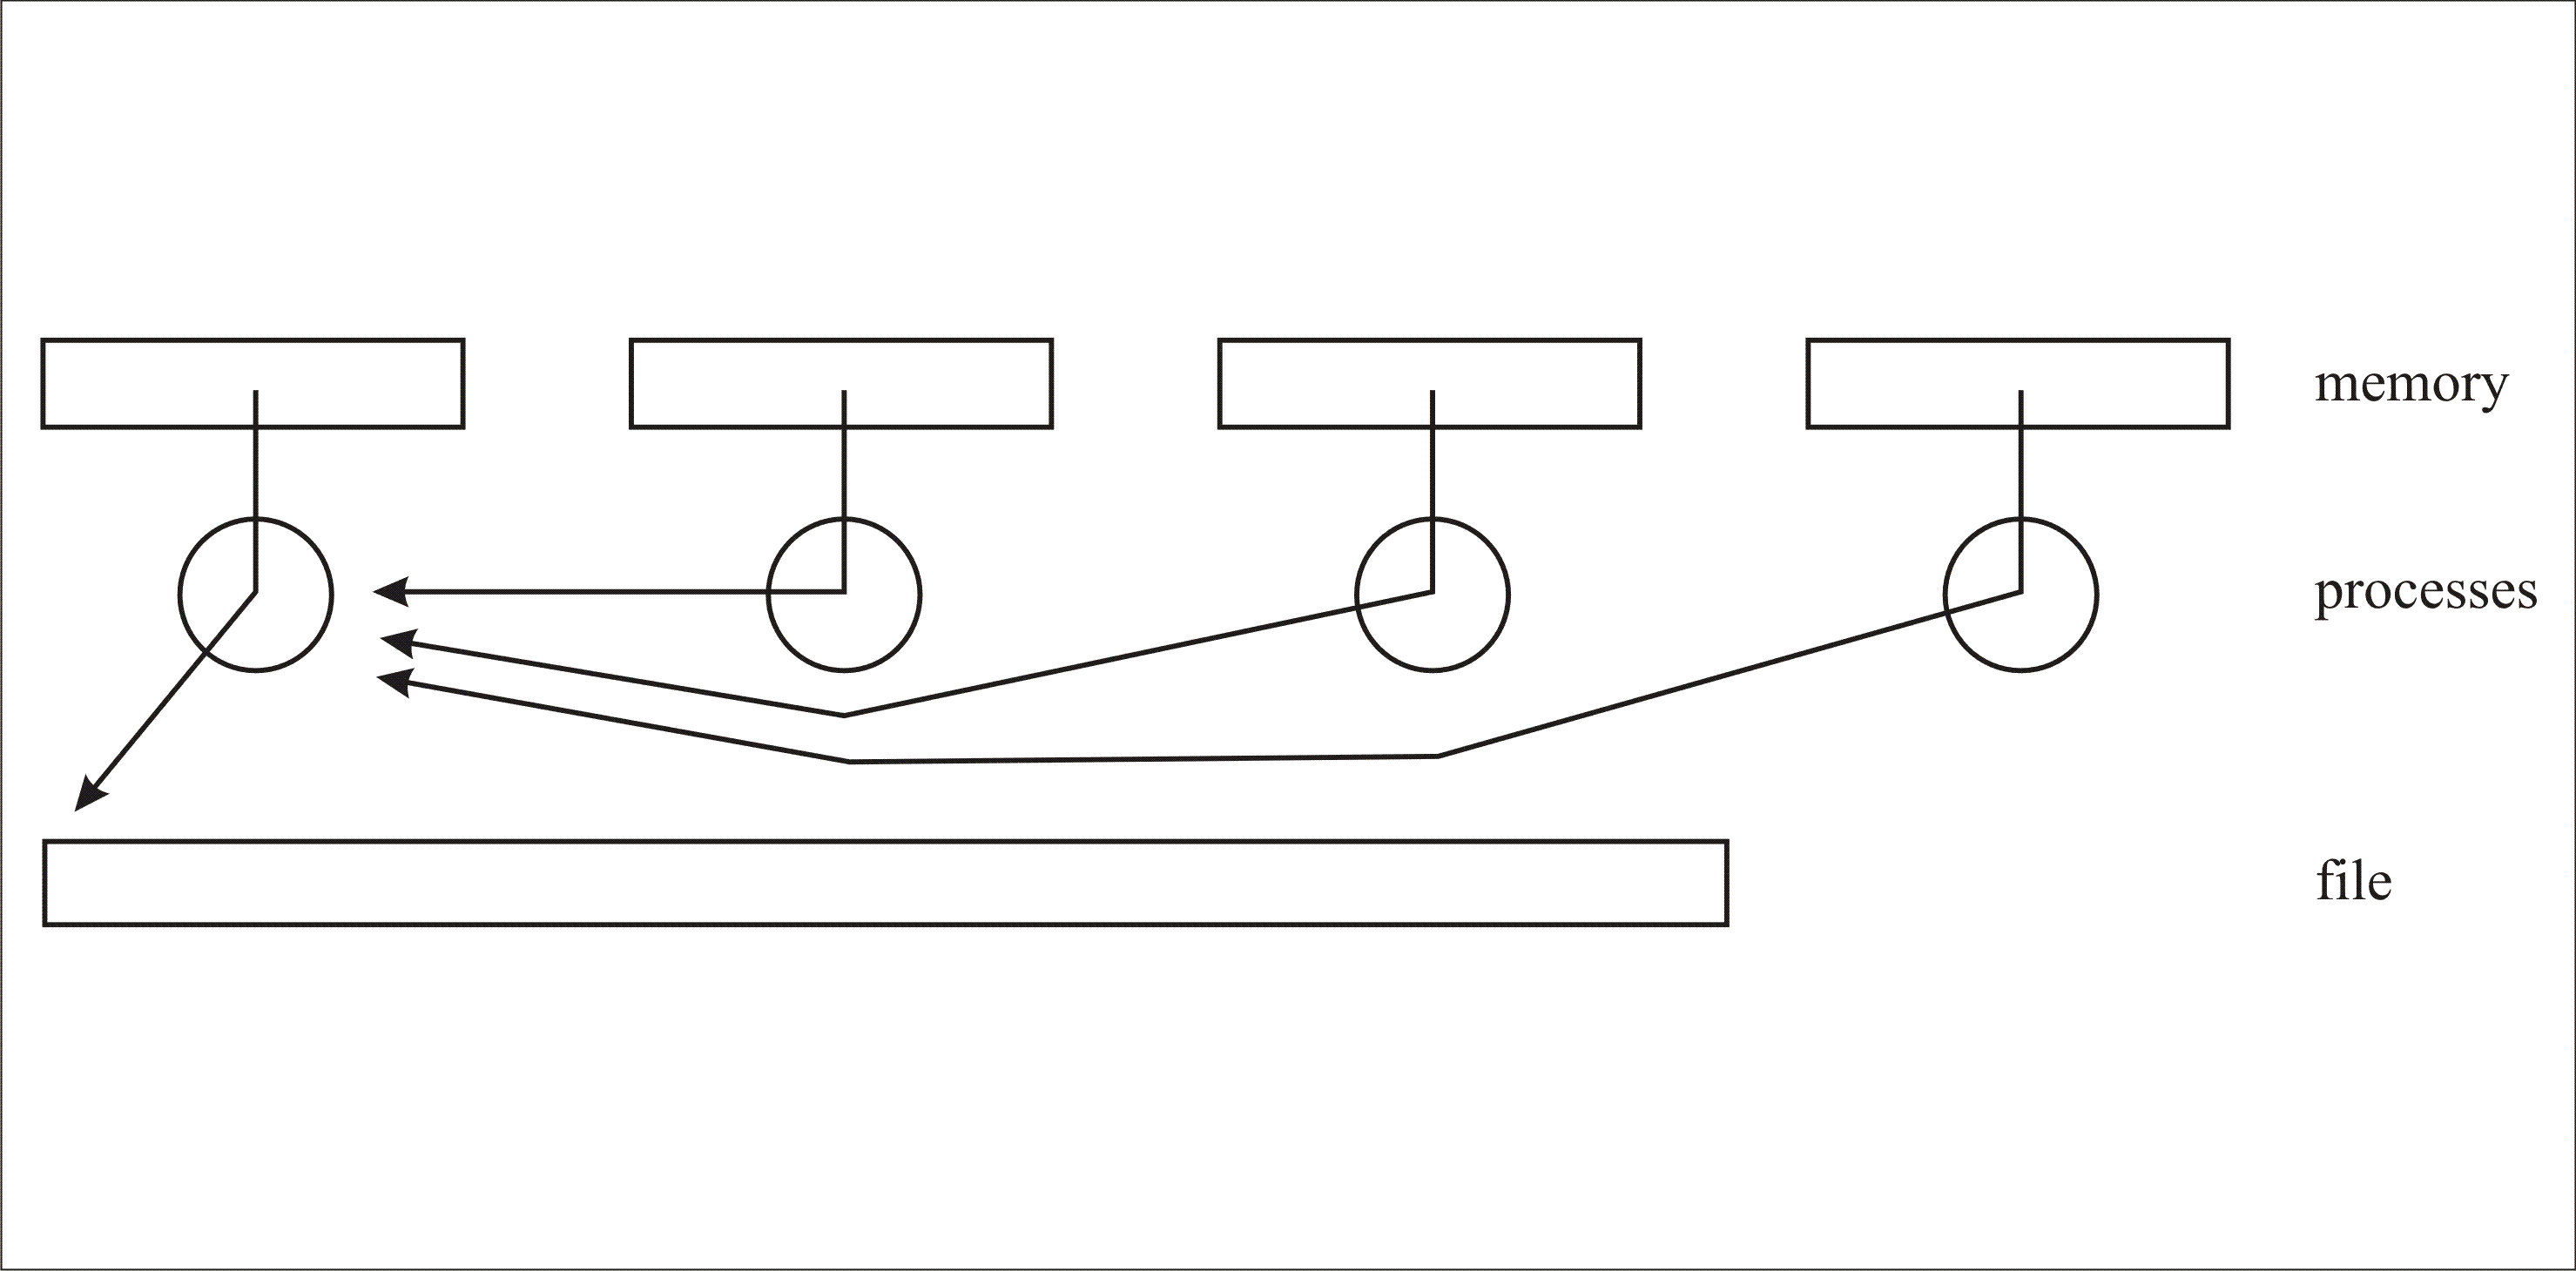
\includegraphics[width=1\textwidth]{slike/sequential_i_o.png}\\[1cm]
  \caption{Секвенцијалне улазно/излазне операције паралелног програма}
\end{figure}

\subsection{MPI програм - непаралелне У/И операције}

MPI-1 нема никакву експлицитну подршку за паралелне У/И операције, док су MPI апликације развијене у последњих неколико година морале да имају и свој У/И део програма. Ти делови програма су писани ослањајући се на карактеристике које пружа оперативни систем, најчешће UNIX. Најједноставније је имати један процес који извршава све У/И операције, док други процеси извршавају операције са учитаним подацима. Ако се узме пример писања низа бројева у фајл дужине 100, онда дужина података коју обрађује сваки процес зависи од укупног броја процеса. Програм почиње иницијализацијом дела низа за сваки процес. Сви процеси осим процеса 0 шаљу своје делове низа процесу 0. Процес 0 уписује свој део низа у фајл, а затим прихвата делове низа од других процеса. Ранг сваког процеса је одређен у  \texttt{MPI\_Recv} функцији, тако да се зна редослед пристизања делова низа. Ово је најчешћи начин да се непаралелне У/И операције врше у паралелном програму који је конвертован из секвенцијалног програма, јер промене нису  направљене на У/И делу програма. 

Уколико је $numprocs=1$, онда нема MPI комуникације. 

Неки од разлога зашто се У/И операције пишу на овај начин су:

\begin{itemize}
\item  Паралелни компјутери на којима је покренут програм можда подржавају У/И операције само са једног процеса.
\item Могу се користити софистициране У/И библиотеке које су можда писане као део високог нивоа слоја за управљање података, а које не подржавају паралелне У/И операције.
\item Резултујући фајл је погодан за руковање изван програма (нпр. \textit{mv}, \textit{cp}, или \textit{ftp}).
\end{itemize}

Учинак програма може бити побољшан омогућавањем процеса да складишти велики блок података. Уколико процес 0 има довољан бафер за податке, он може акумулирати податке других процеса у једниствен бафер за једну велику операцију писања(Листинг 2.1). Разлог због кога не треба писати У/И операције на овај начин је недостатак паралелизма који ограничава учинак и скалабилност, нарочито ако основни систем фајлова омогућава паралелне У/И операције.

\begin{lstlisting}[style=nonumbers,frame=single,language=C, caption= MPI програм ]
#include "mpi.h"
#include <stdio.h>
#define BUFSIZE 100
int main(int argc, char *argv[])
{
	int i, myrank, numprocs, buf[BUFSIZE];
	MPI_Status status;
	FILE *myfile;
	MPI_Init(&argc, &argv);
	MPI_Comm_rank(MPI_COMM_WORLD, &myrank);
	MPI_Comm_size(MPI_COMM_WORLD, &numprocs);

	for (i=0; i<BUFSIZE; i++)
	{
		buf[i] = myrank * BUFSIZE + i;
	}
	if (myrank != 0)
	{
		MPI_Send(buf, BUFSIZE, MPI_INT, 0, 99, MPI_COMM_WORLD);
	}
	else
	{
		myfile = fopen("testfile", "w");
		fwrite(buf, sizeof(int), BUFSIZE, myfile);
		for (i=1; i<numprocs; i++)
		{
			MPI_Recv(buf, BUFSIZE, MPI_INT, i, 99, MPI_COMM_WORLD,
			&status);
			fwrite(buf, sizeof(int), BUFSIZE, myfile);
		}
		fclose(myfile);
	}
	MPI_Finalize();
	return 0;
}
\end{lstlisting}

\subsection{MPI програм - без MPI улазно/излазних операција}
У циљу решавања овог недостатка, следећи корак у миграцији секвенцијалног програма ка паралелном је да се за сваки процес оперише са посебним фајлом, што омогућава паралелни пренос података(Листинг 2.2). Овде су У/И операције сваког процеса потпуно независне од У/И операција других процеса. Тако, је сваки програм секвенцијалан у односу на У/И операције. Наиме, процес отвара свој фајл, уписује податке у њега, а затим га и затвара. Најбоље је да се у називу излазног фајла налази и ранг процеса. Предност овог приступа је да се У/И операције могу одвијати паралелно, а и даље се могу користити секвенцијалне У/И библиотеке. Основни недостатак оваквог приступа је креирање више фајлова уместо једног. Поред тога, недостаци овакве шеме су:

\begin{itemize}
\item Фајлови се морају спојити пре него што буду коришћени као улаз у другом програму.
\item Може се десити да програм који чита ове фајлове мора бити паралелни и стартован са истим бројем процеса.
\item Тешко је држати скуп фајлова као групу, ради копирања, премештања и слања путем мреже.

\end{itemize}

\begin{lstlisting}[style=nonumbers,frame=single,language=C,caption= MPI програм без MPI улазно/излазних операција]
#include "mpi.h"
#include <stdio.h>
#define BUFSIZE 100
int main(int argc, char *argv[])
{
	int i, myrank, buf[BUFSIZE];
	char filename[128];
	FILE *myfile;
	MPI_Init(&argc, &argv);
	MPI_Comm_rank(MPI_COMM_WORLD, &myrank);
	for (i=0; i<BUFSIZE; i++)
	{
		buf[i] = myrank * BUFSIZE + i;
	}
	sprintf(filename, "testfile.%d", myrank);
	myfile = fopen(filename, "w");
	fwrite(buf, sizeof(int), BUFSIZE, myfile);
	fclose(myfile);
	MPI_Finalize();
	return 0;
}
\end{lstlisting}


Учинак може бити мањи уколико имамо велики број процеса. То ће довести до великог броја У/И операција са малим бројем података. 

\subsection{MPI У/И операције са одвојеним фајловима}
MPI У/И програм је сличан као и претходни програм, с тим што се све У/И операције извршавају MPI функцијама(Листинг 2.3). Овакав програм има неколико предности и мана.
 
Прва разлика је у овим фајловима је та што је декларација \texttt{FILE} замењена са \texttt{MPI\_File} као типом \textit{myfile}. Сада је \textit{myfile} променљива типа MPI\_File, уместо показивач на објекат типа FILE.

\begin{lstlisting}[style=nonumbers,frame=single,language=C, caption= MPI програм са одвојеним фајловима]
#include "mpi.h"
#include <stdio.h>
#define BUFSIZE 100
int main(int argc, char *argv[])
{
	int i, myrank, buf[BUFSIZE];
	char filename[128];
	MPI_File myfile;
	MPI_Init(&argc, &argv);
	MPI_Comm_rank(MPI_COMM_WORLD, &myrank);
	for (i=0; i<BUFSIZE; i++)
	{
		buf[i] = myrank * BUFSIZE + i;
	}
	sprintf(filename, "testfile.%d", myrank);
	MPI_File_open(MPI_COMM_SELF, filename,
	MPI_MODE_WRONLY | MPI_MODE_CREATE,MPI_INFO_NULL, &myfile);
	MPI_File_write(myfile, buf, BUFSIZE, MPI_INT,
	MPI_STATUS_IGNORE);
	MPI_File_close(&myfile);
	MPI_Finalize();
	return 0;
}
\end{lstlisting}


MPI функција која замењује функцију fopen назива се \texttt{MPI\_File\_open}.

\begin{verbatim}
MPI_File_open(MPI_COMM\_SELF, filename,MPI_MODE_CREATE | MPI_MODE_WRONLY,
MPI_INFO_NULL, &myfile);
\end{verbatim}

Аргументи ове функције су:

\begin{itemize}
\item \textbf{Комуникатор} - Ovo je најзначајнија компонента У/И операција у MPI. Фајлови су отворени скупом процесора идентификованих од стране комуникатора. 
Ово обезбеђује да процеси раде на фајлу заједно омогућујући и комуникацију између процеса. 
Пошто сваки процес отвара свој фајл, онда се користи комуникатор \texttt{MPI\_COMM\_SELF}.

\item \textbf{Назив фајла} - Други аргумент је стринг који представља назив фајла као и у функцији \textit{fopen}.

\item \textbf{Тип мода} - Трећи аргумент је мод у коме је фајл отворен. У овом програму значи да је креиран или преписан ако већ постоји, као и да ће писање у фајл бити извршено само од стране овог програма. Константе  \texttt{MPI\_MODE\_CREATE} и \texttt{MPI\_MODE\_WRONLY} представљају заставице.

\item  \textbf{MPI\_INFO\_NULL} - MPI\_INFO\_NULL је предефинисана константа која представља лажну вредност за инфо аргумент \texttt{MPI\_File\_open}. 

\item \textbf{Фајл променљива} - Као последњи аргумент је адреса \texttt{MPI\_File} променљиве, коју ће функција \texttt{MPI\_File\_open} отворити. Као и све MPI функције у C програму, \texttt{MPI\_File\_open} има повратну вредост. Уколико је фајл успешно отворен повратна вредност је \texttt{MPI\_SUCCESS}.

\end{itemize}
 
Следећа функција која је важна за функционисање за MPI У/И је:

 \begin{verbatim}
MPI_File_write(myfile, buf, BUFSIZE, MPI_INT,MPI_STATUS_IGNORE);
\end{verbatim}

Податак који се уписује мора бити одређен адресом, величином и типом. Овим начином се описује бафер који ће бити коришћен за писање(Листинг 2.4). То омогућава да се несуседни подаци у меморији запишу само једним позивом. Конкретно, овде се уписују 
\texttt{BUFSIZE} целих бројева са почетком у адреси \textit{buf}. Последњи аргумент функције је статус, који је истог типа као и код \texttt{MPI\_Recv}.
У овом сличају занемариће се повратна вредност. MPI-2 је одредио специјалну вредност статуса \texttt{MPI\_STATUS\_IGNORE}. Ова вредност може бити послата ако аргумент било којој MPI функцији у циљу игнорисања повратне вредности одговарајуће функције.
Технички, ово упрошћење може побољшати учинак програма уколико нам статус није потребан.

Функција \texttt{MPI\_File\_close(\&myfile)} служи за затварање фајла. Послата адреса \textit{myfile} биће преписана са  \texttt{MPI\_FILE\_NULL} уколико се затварање фајла не обави успешно. Тако се могу идентификовати неважећи фајлови.

\begin{lstlisting}[style=nonumbers,frame=single,language=C, caption=MPI програм за паралелним MPI функцијама]
#include "mpi.h"
#include <stdio.h>
#define BUFSIZE 100
int main(int argc, char *argv[])
{
	int i, myrank, buf[BUFSIZE];
	MPI_File thefile;
	MPI_Init(&argc, &argv);
	MPI_Comm_rank(MPI_COMM_WORLD, &myrank);
	for (i=0; i<BUFSIZE; i++)
	{
		buf[i] = myrank * BUFSIZE + i;
	}
	MPI_File_open(MPI_COMM_WORLD, "testfile",
	MPI_MODE_CREATE | MPI_MODE_WRONLY,
	MPI_INFO_NULL, &thefile);
	MPI_File_set_view(thefile, myrank * BUFSIZE * sizeof(int),
	MPI_INT, MPI_INT, "native", MPI_INFO_NULL);
	MPI_File_write(thefile, buf, BUFSIZE, MPI_INT,
	MPI_STATUS_IGNORE);
	MPI_File_close(&thefile);
	MPI_Finalize();
	return 0;
}
\end{lstlisting}


\subsection{Паралелне MPI У/И операције са једним фајлом}

Да би се добио још бољи учинак MPI У/И операција, потребно је изменити програм тако да процеси деле један фајл, уместо да пишу у више њих(слика 2.2). Тако се отклањају све мане код уписа у више фајлова и постиже се потпуни паралелизам.

Прва разлика између програма који уписује у више различитих фајлова је први аргумент функције \texttt{MPI\_File\_open}. Пошто сада сваки процес не приступа свом фајлу, већ једном дељеном за све процесе, уместо комуникатора \texttt{MPI\_COMM\_SELF} користи се комуникатор  \texttt{MPI\_COMM\_WORLD}. Тиме се постиже да сви процеси отварају исти фајл.

\begin{figure}[h!]
  \centering
      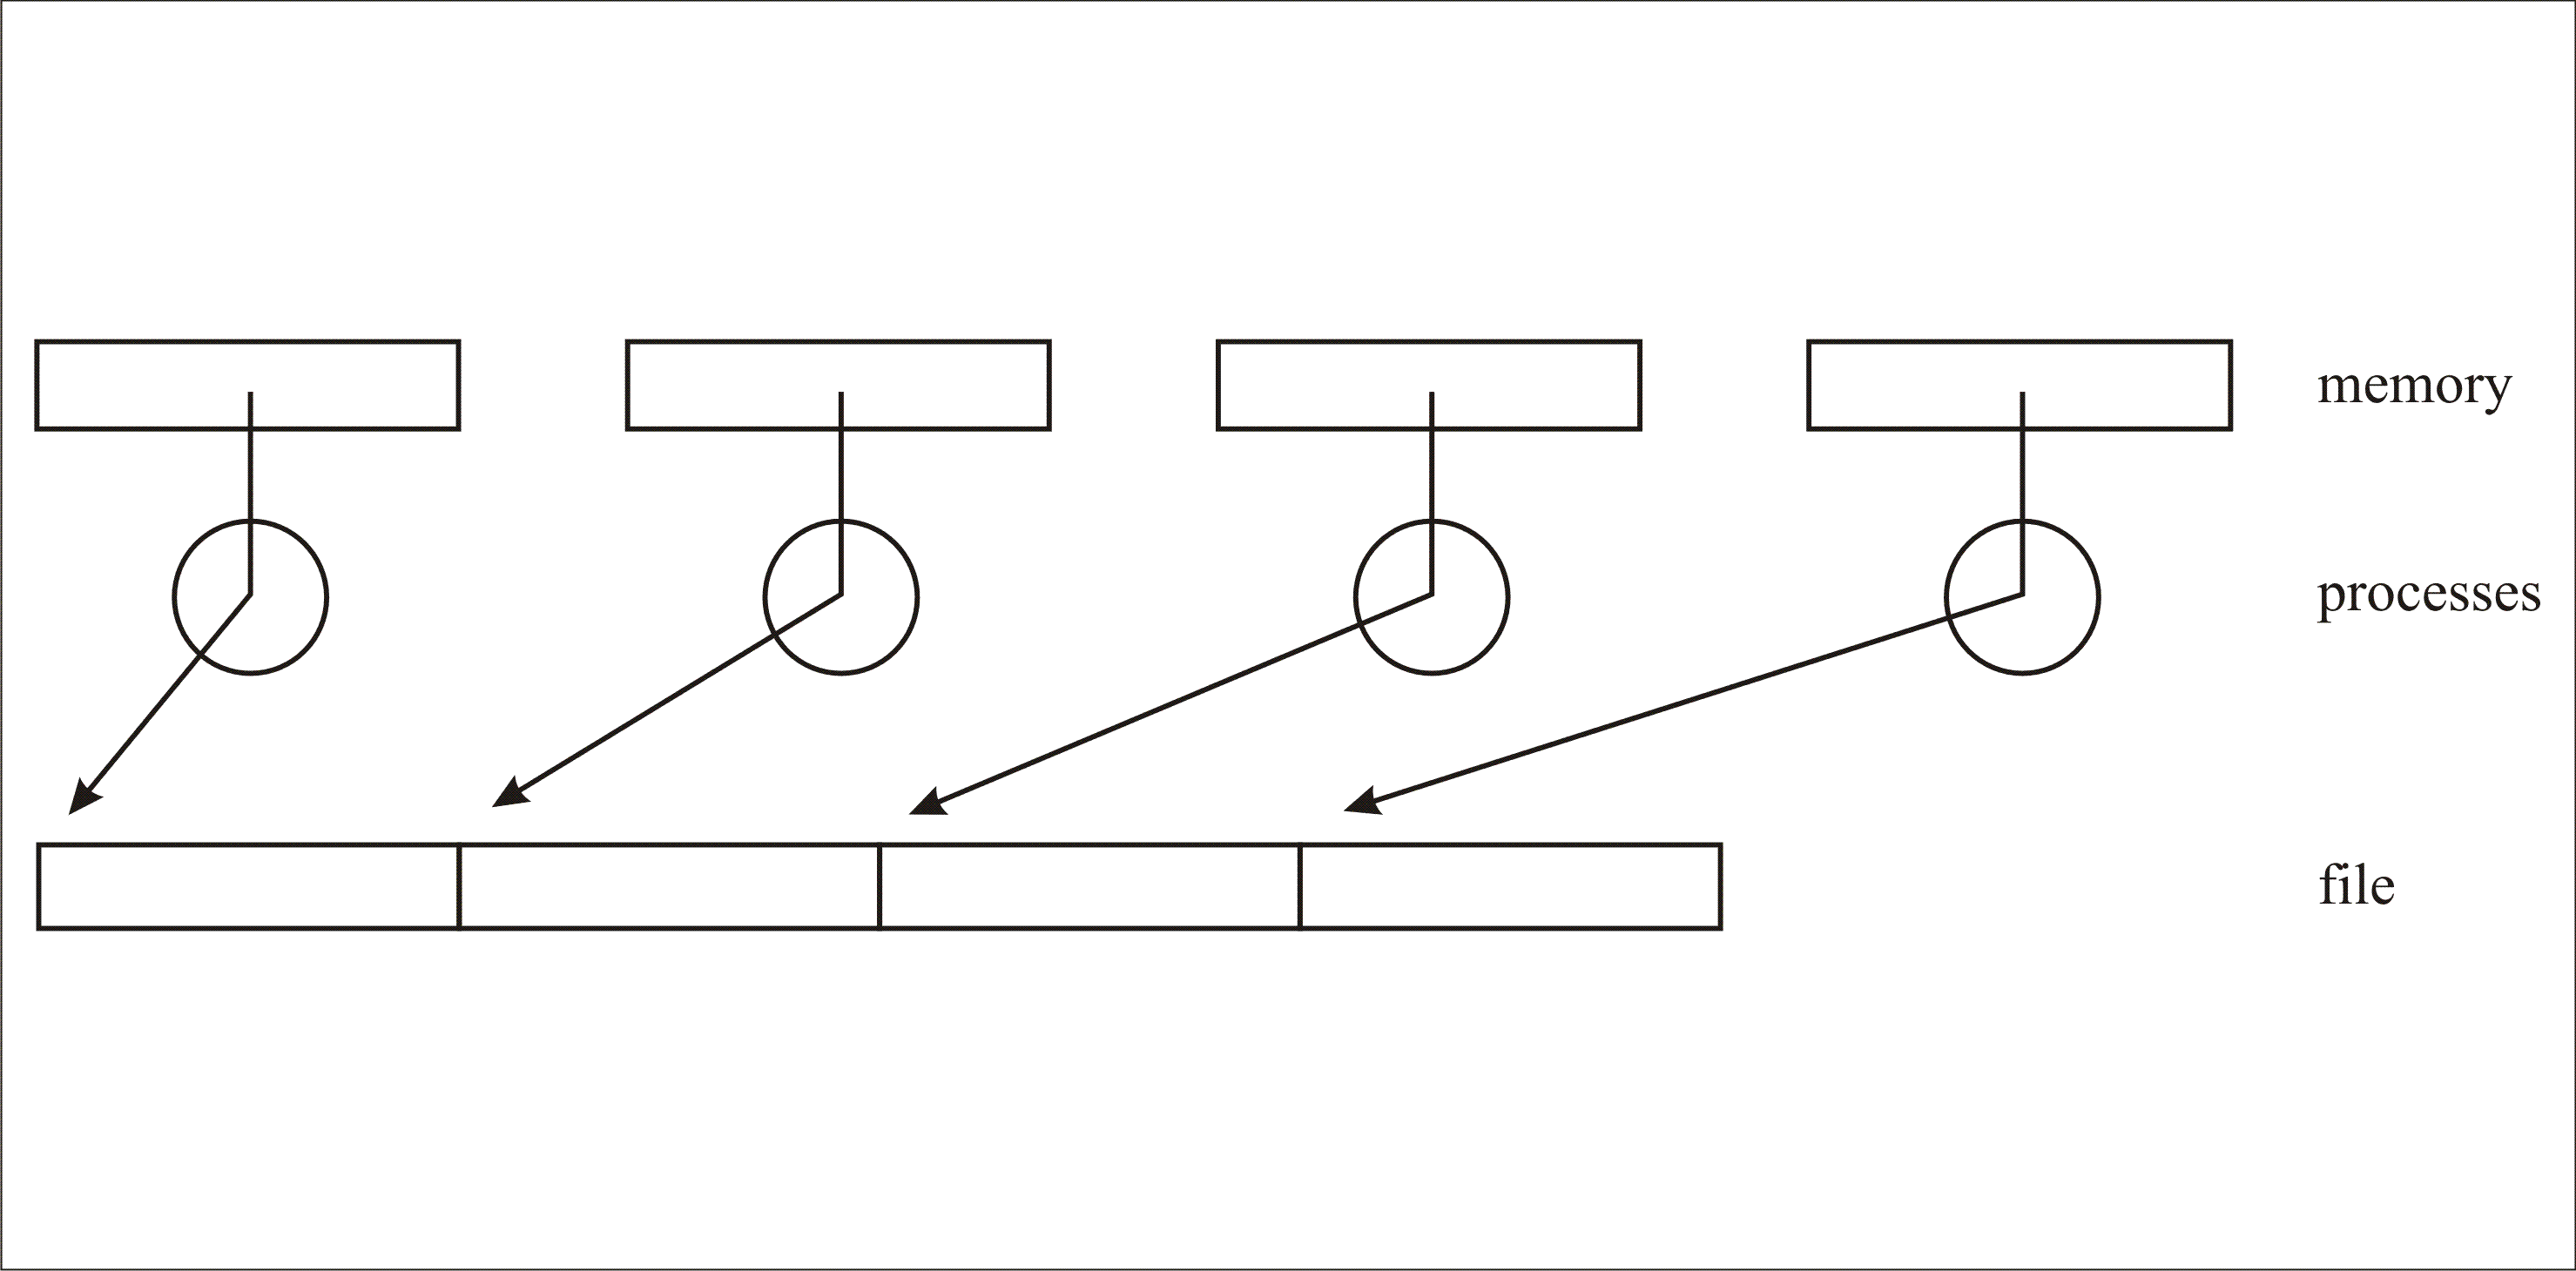
\includegraphics[width=1\textwidth]{slike/paralel_i_o_single_file.png}\\[1cm]
  \caption{Паралелне MPI У/И операције са једним фајлом}
\end{figure}

Ово је колективна операција  на комуникатору, тако да сви процеси који учествују позивају \texttt{MPI\_File\_open}, при чему се, као што је напоменуто, отвара се само један фајл. Део фајла може се видети у процесу, што се назива \textbf{поглед фајла}. Поглед фајла се поставља функцијом \texttt{MPI\_File\_set\_view}.

\begin{verbatim}
MPI_File_set_view(thefile, myrank * BUFSIZE * sizeof(int), MPI_INT,
 MPI_INT, "native", MPI_INFO_NULL);
\end{verbatim}

Први аргумент идентификује фајл. Други аргумент је место (у бајтовима) у фајлу од кога почиње део фајла асоциран датом процесу.
Овде множимо величину података (BUFSIZE * sizeof (int)) по рангу процеса, тако да поглед на сваки процес почиње на одговарајућем месту у фајлу.
Тај аргумент је типа \texttt{MPI\_Offset}, који на системима који подржавају велике фајлове очекује 64-битни цели број. Следећи аргумент се назива \textbf{etype погледа}. То је скуп свих типова података који се налазе у фајлу. У овом случају то је \texttt{MPI\_INT}, што значи да ће се у фајл увек уписати цели број. Следећи аргумент се назива \textit{filetype}, и то је веома флексибилан начин да се опишу дисконтинуални погледи у фајлу. У овом случају ради се само о типу \texttt{MPI\_INT}, тако да нема дисконтинуалних података за упис. Генерално, \textit{etype} и \textit{filetype} могу да буду било који предефинисани MPI типови података. Аргумент који означава представљање података у фајлу и најчешће је типа стринг назива се \zn природни". Нативно представљање значи да се подаци уписују у фајл тачно онако како су представљени у меморији. Ова шема чува податке и сумарни учинак програма, јер се не губи време ни на какве додатне конверзије.
Остала представљања су \textit{унутрашња} и \textit{external32}, која омогућавају различите врсте преноса између машина са различитим архитектурама и типовима представљања.
Последњи аргумент је инфо аргумент као и у функцији \texttt{MPI\_File\_open}.

Неке MPI функције у програмском језику C се налазе у Листингу 2.5:

\begin{lstlisting}[style=nonumbers,frame=single, language=C, caption=MPI функције]
int MPI_File_open(MPI_Comm comm, char *filename, int amode, MPI_Info info,
MPI_File *fh)

int MPI_File_set_view(MPI_File fh, MPI_Offset disp, MPI_Datatype etype,
MPI_Datatype filetype, char *datarep, MPI_Info info)

int MPI_File_write(MPI_File fh, void *buf, int count, MPI_Datatype datatype,
MPI_Status *status)
int MPI_File_close(MPI_File *fh)

int MPI_File_get_size(MPI_File fh, MPI_Offset *size)
int MPI_File_read(MPI_File fh, void *buf, int count, MPI_Datatype datatype,
MPI_Status *status)
\end{lstlisting}

Овим начином, написани програм је независан од броја процеса на којима је покренут. Укупна величина датотеке се добија тако да сваки процес ради са скоро истом величином података.
MPI функција која се користи за добијање величине фајла је  \texttt{MPI\_File\_get\_size}. Први аргумент ове функције је отворени фајл, а другi je адреса где треба сместити израчунату величину фајла у бајтовима. Пошто многи системи сада могу управљати датотекама чије су дужине превелике да би биле
представљене као 32-битни цео број, MPI дефинише тип,  \texttt{MPI\_Offset}, који може да а садржи величину фајла у 64 бита. 
То је тип који се користи 
за аргументе MPI функција који се односе на померање у фајловима. У супротном, програм који се користи за читање фајла је веома сличан оном који пише. Разлика између писања и читања је да процес не зна увек тачно колико ће података буде прочитано.

\subsection{Коришћење појединачних фајл показивача}

MPI програм са улазно/излазним операцијама је могуће писати и са појединачним фајл показивачима(Листинг 2.6). Сваки од ових програма има део за У/И операције које отварају, читају и на крају затварају фајл. \texttt{MPI\_File\_open} је функција која отвара фајл. Први аргумент је комуникатор који идентификује групу процеса којима је потребан приступ фајлу. \texttt{MPI\_COMM\_WORLD} се користи зато што је свим процесима потребан приступ фајлу \textit{/pfs/datafile}. MPI стандард не одређује формат за назив фајла. Свака од MPI имплементација има слободу да дефинише формат који они подржавају. Може се очекивати да ће имплементација подржати познате конвенције именовања. Имплементације које се покрећу на Unix окружењу подржавају Unix конвенцију именовања. \textit{/pfs/datafile} је фајл који се налази у директоријуму \textit{pfs}. У имплементацијама је назив директоријума опциони део назива фајла. Уколико не постоји, имплементација ће користити директоријум у коме се процес тренутно налази. Трећи аргумент функције \texttt{MPI\_File\_open} је начин приступа. У овом сличају то је \texttt{MPI\_MODE\_RDONLY}, зато што је довољно да програм само чита из фајла. Четврти аргумент је инфо аргумент. Последњи аргумент је показивач на фајл који враћа функција \texttt{MPI\_File\_open}.


\begin{lstlisting}[style=nonumbers,frame=single,language=C, caption= MPI програм са појединачним фајл показивачима]
#include "mpi.h"
#define FILESIZE (1024 * 1024)
int main (int argc, char **argv)
{
int *buf, rank, nprocs, nints, bufsize;
MPI_File fh;
MPI_Status status;
MPI_Init(&argc,&argv);
MPI_Comm_rank(MPI_COMM_WORLD, &rank);
MPI_Comm_size(MPI_COMM_WORLD, &nprocs);
bufsize = FILESIZE/nprocs;
buf = (int *) malloc (bufsize);
nints = bufsize/sizeof (int);
MPI_File_open(MPI_COMM_WORLD, "/pfs/datafile", MPI_MODE_RDONLY,
MPI_INFO_NULL, &fh);
MPI_File_seek(fh, rank*bufsize, MPI_SEEK_SET);
MPI_File_read(fh, buf, nints, MPI_INT, &status);
MPI_File_close(&fh);
free (buf);
MPI_Finalize();
return 0;
}
\end{lstlisting}

Овај C програм извршава улазно/излазне операције користећи појединачне показиваче на фајл. После отварања фајла, сваки процес копира глобални фајл показивач у локални фајл показивач који показује на локацију у фајлу од које сваки процес чита свој део фајла. Први аргумент функције \texttt{MPI\_File\_seek} је показивач на фајл који је отворила функција 
\texttt{MPI\_File\_open}. Други аргумент одређује део фајла који сваки процес чита. \texttt{MPI\_SEEK\_SET} значи да се почетак локације за читање рачуна од почетка фајла. У C програмском језику 
за ово се користи предефинисан тип \texttt{MPI\_Offset}. Имплементација дефинише \texttt{MPI\_Offset} као цео број који је довољно велики да подржи највећу дужину фајла. Део фајла сваког процеса се одређује производом ранга процеса и величине податка у бајтовима. Величина податка може се одредити и функцијама \texttt{MPI\_Get\_countor} \texttt{MPI\_Get\_elements}, користећи статус објекат који враћа функција \texttt{MPI\_File\_read}.


\subsection{Употреба експлицитних одступања}

\texttt{MPI\_File\_read} и \texttt{MPI\_File\_write} се називају појединачним фајл показивачима због тога што користе показивач на локацију у фајлу од које сваки процес чита фајл(Листинг 2.7). MPI такође специфицира  неколико функција које се називају \textbf{експлицитним функцијама одступања} (\texttt{MPI\_File\_read\_at} и \texttt{MPI\_File\_write\_at}). Ове функције не користе појединачне фајл показиваче. У њима, локација у фајлу се директно прослеђује функцији као аргумент. Уколико више нити процеса приступају истом фајлу, онда се морају користити појединачни фајл показивачи због безбедности нити.

\begin{lstlisting}[style=nonumbers,frame=single,language=C, caption= MPI функције]
int MPI_File_read_at(MPI_File fh, MPI_Offset offset, void *buf, int count,
MPI_Datatype datatype, MPI_Status *status)
int MPI_File_write_at(MPI_File fh, MPI_Offset offset, void *buf, int count,
MPI_Datatype datatype, MPI_Status *status)
\end{lstlisting}

\subsection{Писање у фајл}
Уколико је потребно уписати податке у фајл, онда се користе функције \texttt{MPI\_File\_write} и \texttt{MPI\_File\_write\_at}. Уместо заставице \texttt{MPI\_MODE\_RDONLY} која је служила за читање фајла, за упис података у фајл се користе заставице \texttt{MPI\_MODE\_CREATE} и \texttt{MPI\_MODE\_WRONLY}. \texttt{MPI\_MODE\_CREATE} се користи за креирање фајла уколико он већ не постоји. \texttt{MPI\_MODE\_WRONLY} означава да је фајл отворен за писање. У C програмском језику, обе заставице могу се користити битовним или оператором :  \texttt{MPI\_MODE\_CREATE} | \texttt{MPI\_MODE\_WRONLY}. Да би функција \texttt{MPI\_File\_open} креирала фајл, потребно је да постоји директоријум који је наведен у називу фајла.

\subsection{Неконтинуални приступи и колективне У/И операције}

У великом броју реалних паралелних апликација, сваком процесу је потребно да приступи малим деловима података који су смештени у фајлу неконтинуално  [4, 17, 65, 77, 78, 85].
Један начин да се приступи неконтунуалним подацима је користећи функције за читање/писање малих континуалних делова, као у Unix системима. Због велике латенције улазно/излазних операција, приступање малим деловима података захтева много времена. Предност MPI на Unix системима је могућност приступа неконтинуалним деловима података позивајући само једну функцију. 

\subsubsection{Неконтинуални приступи}
MPI програм поседује концепт погледа на фајл. Поглед фајла у MPI-у је дефинисан као део фајла коме процес има приступ(слика 2.3). Користећи поглед на фајл, функције читања и писања могу приступити само том делу фајла. Сви остали подаци се прескачу. Када се отвори, фајл је доступан процесу и MPI третира фајл као скуп бајтова (не као цели бројеви, реални бројеви итд.). Приликом покретања програма, сваки пројединачни фајл показивач је постављен на 0. Ово се може променити помоћу функције \texttt{MPI\_File\_set\_view}(Листинг 2.8). Најчешће се то ради из два разлога:

\begin{itemize}
\item Да се одреди тип податка коме је потребно приступити, нпр. целим или децималним бројевима. 
Ово је нарочито неопходно за преносивост фајла уколико корисник жели да приступи фајлу са друге машине и са различитим представљањем фајла. 

\item Да се одреде делови фајла који ће бити прескочени, тј. одређивање неконтунуалног приступа фајлу. За појединачне фајл показиваче или експлицитна одступања, сваки процес може користети различит тип погледа.
\end{itemize}

За приступ подацима са подељеним фајл показивачем потребно је да сви процеси користе исти поглед. Поглед фајла се може мењати небројано пута.
MPI типови података се користе за одређивање погледа фајла. Поглед је одређен са:

\begin{itemize}
\item премештање
\item \textit{etype}
\item \textit{filetype}
\end{itemize}

\textbf{Премештање} одређује број бајтова који ће бити прескочени на почетку фајла. Ово се користи када је потребно да се прескочи читање заглавља фајла.
\textbf{Еtype} је основна јединица за приступ подацима. Може бити основни или изведени MPI тип података. Сви приступи фајлу се врше преко јединица типа etype. Сва одступања фајла се дефинишу као број \textit{ etype-ова}. Уколико је \textit{etype} MPI\_INT, појединачни и подељен фајл показивач биће померен за одређени број целих бројева.
\textbf{Filetype} je основни или изведени тип података који дефинише који део фајла је доступан процесу и ког типа су подаци. \textit{Filetype} мора бити исти као etype или изведен од типа који се заснива на \textit{etype}.
Поглед фајл почиње од премештања и састоји се од више суседних \textit{etype}. Приликом отварања фајла, премештање има вредност 0  и \textit{etype} и \textit{filetype} су типа \texttt{MPI\_BYTE}. Ово је познато као подразумевани поглед фајла. 

\begin{figure}[h!]
  \centering
      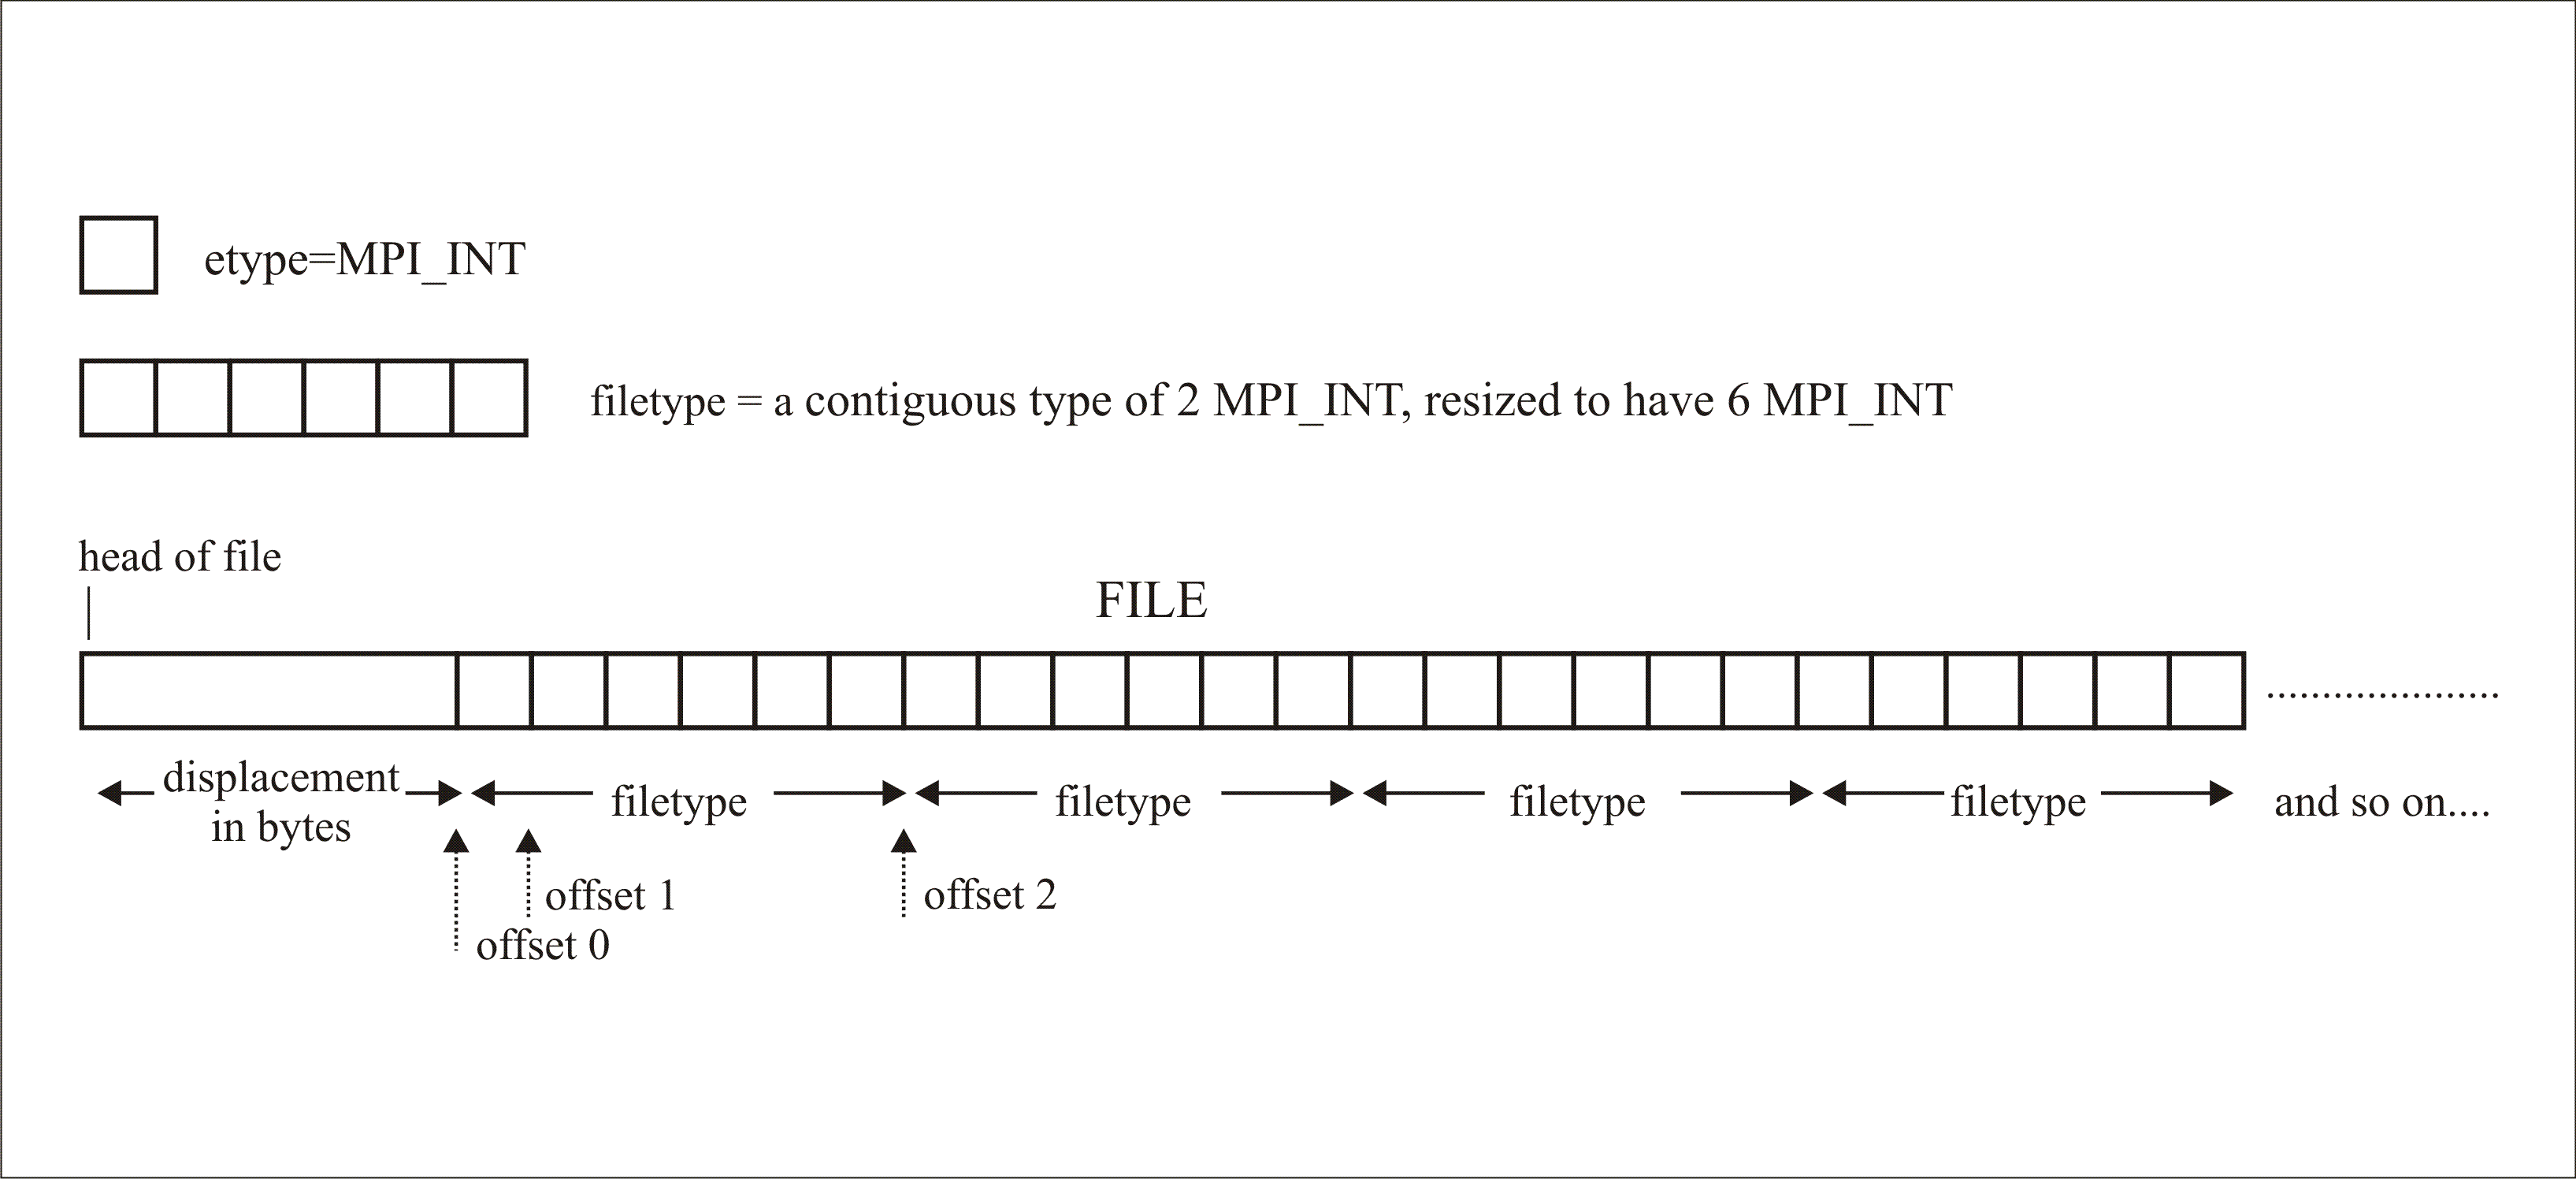
\includegraphics[width=1\textwidth]{slike/displacement.png}\\[1cm]
  \caption{Поглед фајла}
\end{figure}

На слици 2.3 је приказан суседни изведени тип података који је представљен као два цела броја. Уколико се поставе још 4 цела броја на крај овог типа података, функцијом\texttt{ MPI\_Type\_create\_resized} се добија тип податка који је величине шест целих бројева. \texttt{Еtype} је типа \texttt{MPI\_INT}, а премештање је 5*sizeof (int). У MPI-1 верзији ово се ради са функцијом \texttt{MPI\_Type\_struct}.

\begin{lstlisting}[style=nonumbers,frame=single, language=C, caption= MPI функције]
int MPI_File_set_view(MPI_File fh, MPI_Offset disp, MPI_Datatype etype,
MPI_Datatype filetype, char *datarep, MPI_Info info)
int MPI_Type_create_resized(MPI_Datatype oldtype, MPI_Aint lb,
MPI_Aint extent, MPI_Datatype *newtype)
\end{lstlisting}

Аргументи који се прослеђују функцији \texttt{MPI\_File\_set\_view} су:
\begin{itemize}
	\item показивач на фајл
	\item премештање
	\item \textit{etype}
	\item \textit{filetype}
	\item предствљање података
	\item инфо аргумент
\end{itemize}
Подразумевано представљање је нативно, док је подразумевани инфо аргумент \texttt{MPI\_INFO\_NULL}.

\subsubsection{Kолективне У/И операције}

Разлика између колективних У/И операција са неконтинуалним приступом и других У/И операција је у томе што код колективних операција сваки процес чита мале блокове података, који се налазе у фајлу по принципу \textit{round-robin} распоређивања(слика 2.4). Са Unix У/И операцијама, једини начин да се читају подаци је читање сваког блока одвојено, због тога што Unix функције омогућавају приступ само једном континуалном делу података. 

\begin{figure}[h!]
  \centering
      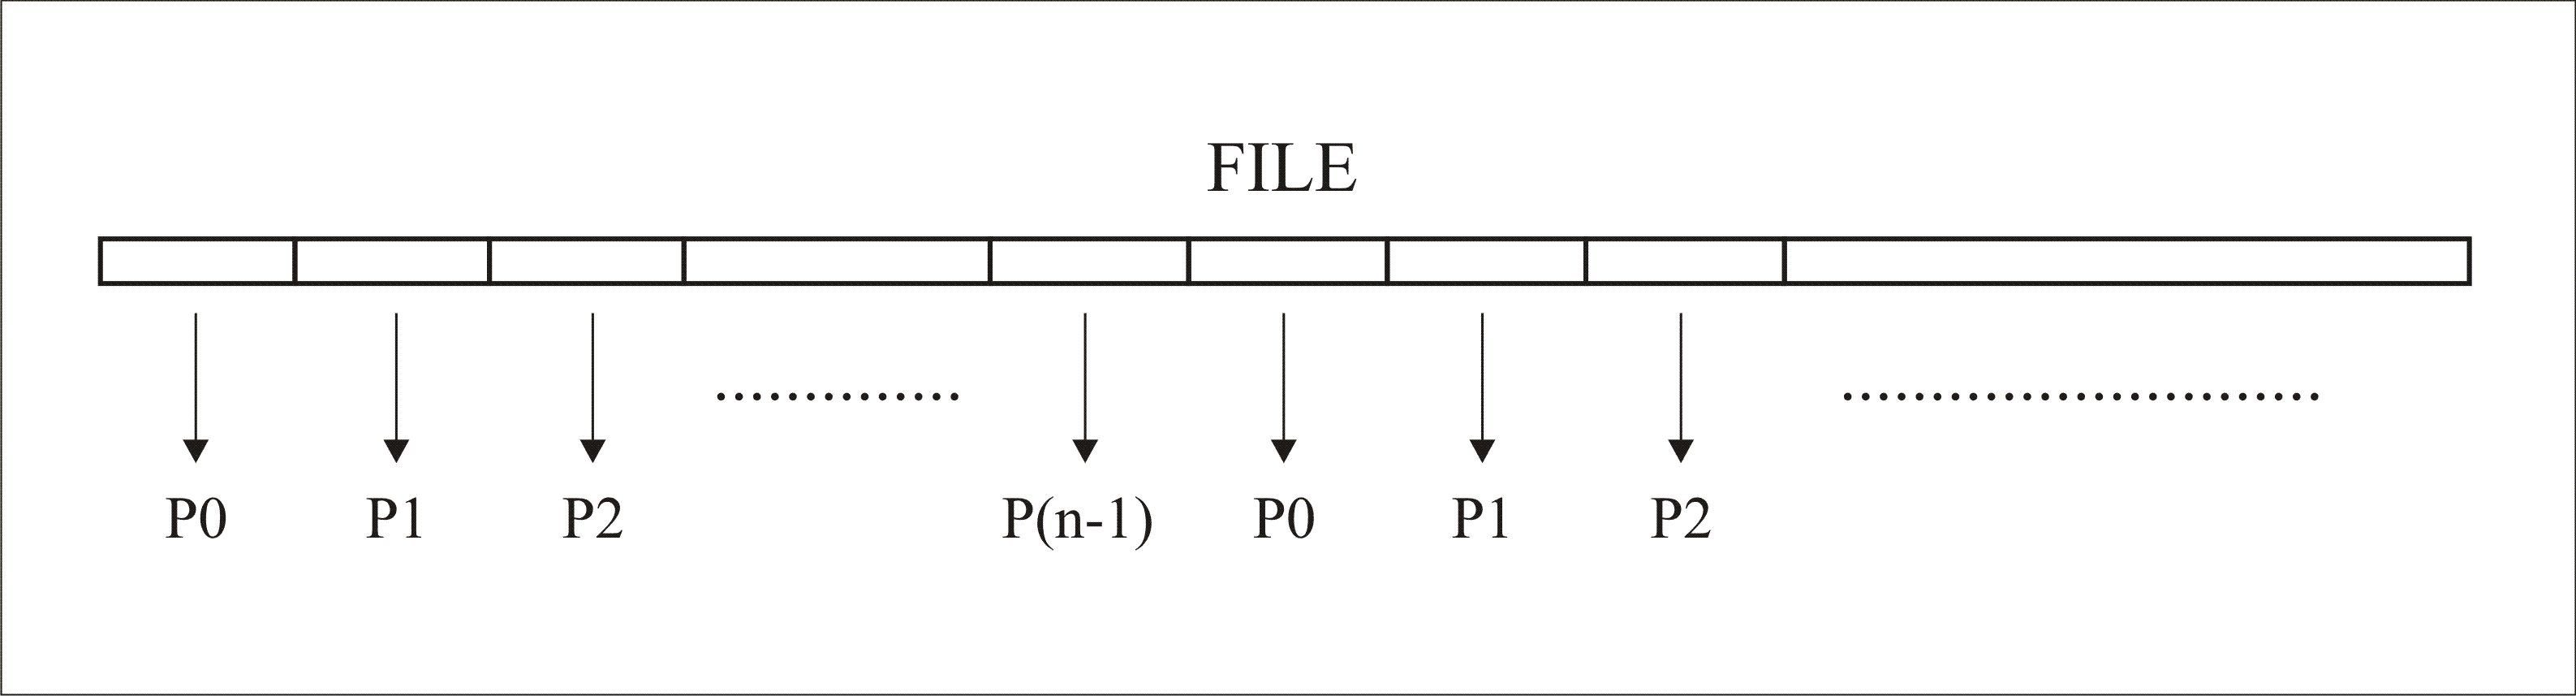
\includegraphics[width=1\textwidth]{slike/block-cyclic.png}\\[1cm]
  \caption{Колективне У/И операције}
\end{figure}

Код MPI-a, уместо позивања функције за читање више пута, може се дефинисати поглед на неконтунуални фајл сваког процеса, како би се прочитао фајл позивајући функцију само једном(Листинг 2,9). Други начин је употреба колективног читања. MPI имплементација даје много бољи учинак у односу на Unix У/И функције.

\texttt{FILESIZE} одређује величину фајла у бајтовима. \texttt{INTS\_PER\_BLK }је величина сваког блока који процес треба да прочита (број целих бројева у блоку). Сваки процес треба да прочита неколико блокова у цикличном распореду.

\begin{lstlisting}[style=nonumbers,frame=single,language=C, caption=MPI програм са погледом фајла]
#include "mpi.h"
#define FILESIZE
#define INTS_PER_BLK 104857616

int main(int argc, char **argv)
{
	int *buf, rank, nprocs, nints, bufsize;
	MPI_File fh;
	MPI_Datatype filetype;
	MPI_Init(&argc,&argv);
	MPI_Comm_rank(MPI_COMM_WORLD, &rank);
	MPI_Comm_size(MPI_COMM_WORLD, &nprocs);
	bufsize = FILESIZE/nprocs;
	buf = (int *) malloc(bufsize);
	nints = bufsize/sizeof(int);
	MPI_File_open(MPI_COMM_WORLD, "/pfs/datafile", MPI_MODE_RDONLY,
	MPI_INFO_NULL, &fh);
	MPI_Type_vector(nints/INTS_PER_BLK, INTS_PER_BLK,
	INTS_PER_BLK*nprocs, MPI_INT, &filetype);
	MPI_Type_commit(&filetype);
	MPI_File_set_view(fh, INTS_PER_BLK*sizeof(int)*rank, MPI_INT,
	filetype, "native", MPI_INFO_NULL);
	MPI_File_read_all(fh, buf, nints, MPI_INT, MPI_STATUS_IGNORE);
	MPI_File_close(&fh);
	MPI_Type_free(&filetype);
	free(buf);
	MPI_Finalize();
	return 0;
}
\end{lstlisting}

Помоћу  \texttt{MPI\_File\_open} отвара се фајл и поставља се комуникатор MPI\_COMM\_WORLD пошто сваки процес треба да има приступ фајлу\textit{ /pfs/datafile}.
Следећи корак је дефинисање погледа. За filetype, креира се изведени тип типа вектор, користећи функцију \texttt{MPI\_Type\_vector}. Први аргумент ове функције је број блокова који сваки процес треба да прочита. Други аргумент је број целих бројева у сваком блоку, док је трећи број целих бројева између полазних елемената два узастопна блока које процес чита. Четврти аргумент је тип податка, у овом случају MPI\_INT. Пети аргумент је повратна вредност функције \texttt{MPI\_Type\_vector}. Након креирања овог типа, нови тип се може користити као \textit{filetype} аргумент функције \texttt{MPI\_File\_set\_view}. 

\textit{Еtype} је \texttt{MPI\_INT}. Улазно/излазне операције се извршавају користећи колективну верзију функције  \texttt{MPI\_File\_read}, која се назива \texttt{MPI\_File\_read\_all}. У позивима ових функција нема разлике. Једина разлика је што се колективна функција позива од стране сваког процеса у комуникатору који је прослеђен функцији \texttt{MPI\_File\_open}. Овај комуникатор је имплицитно прослеђен функцији \texttt{MPI\_File\_read\_all}. Функција \texttt{MPI\_File\_read}, може се позивати независно од стране процеса.


\subsection{Приступни низови  смештени у фајловима}
Велики број паралелних програма има један или више вишедимензионих низова подељених између процеса. Локални низ сваког процеса није контунуално смештен у фајл. Сваки ред низа сваког процеса
је одвојен редовима локалних низова других процеса. MPI омогућава погодан начин за опис улазно/излазних операција и извршава их преко једног позива функције. Уколико корисник користи колективне У/И функције, MPI имплементација омогућава бољи учинак користећи овакав приступ, иако је приступ дисконтунуални. У MPI-2 је дефинисано два нова типа конструктора података: \textbf{darray} и \textbf{subarray}. Ове функције  олакшавају креирање изведених типова података, описујући локацију локалних низова спојених у један глобални низ. Ови типови података могу бити коришћени као filetype да опишу дисконтинуални приступ фајлу, када се обавља У/И операција за подељене низове.

\subsection{Подељени низови}
Конструктор типа података \textit{darray} омогућава лак начин креирања изведеног типа података, који описује мултидимензионални глобални низ који се састоји од локалних низова(слика 2.5). Низ може бити било којих димензија и свака димензија може бити дистрибуирана на било који начин. Аргументи \textit{darray} конструктора су величина низа, опис расподеле  и ранг процеса чији је локални низ описан. Излаз је изведен тип података који описује распоред локалних низова у глобалном низу. Постоје и други начини за креирање изведених типова података, али су они нешто сложенији.
Први аргумент функције \texttt{MPI\_Type\_create\_darray} је број процеса којима је низ дистрибуиран. Други аргумент је ранг процеса чији је локални низ описан. Трећи аргумент су димензије низа, док је четврти аргумент сам низ.

\begin{lstlisting}[style=nonumbers,frame=single,language=C, caption= Део MPI програма са подељеним низовима]
gsizes[0] = m;
gsizes[1] = n;

distribs[0] = MPI_DISTRIBUTE_BLOCK;
distribs[1] = MPI_DISTRIBUTE_BLOCK;

dargs[0] = MPI_DISTRIBUTE_DFLT_DARG; /* default block size */
dargs[1] = MPI_DISTRIBUTE_DFLT_DARG; /* default block size */
psizes[0] = 2;
psizes[1] = 3;

MPI_Comm_rank(MPI_COMM_WORLD, &rank);
MPI_Type_create_darray(6, rank, 2, gsizes, distribs, dargs,
psizes, MPI_ORDER_C, MPI_FLOAT, &filetype);
MPI_Type_commit(&filetype);
MPI_File_open(MPI_COMM_WORLD, "/pfs/datafile",
MPI_MODE_CREATE | MPI_MODE_WRONLY,
MPI_INFO_NULL, &fh);
MPI_File_set_view(fh, 0, MPI_FLOAT, filetype, "native",
MPI_INFO_NULL);
local_array_size = num_local_rows * num_local_cols;
MPI_File_write_all(fh, local_array, local_array_size,
MPI_FLOAT, &status);
MPI_File_close(&fh);
\end{lstlisting} 

Пети аргумент је низ који одређује начин на који је глобални низ подељен. На овом примеру, ту улогу има \texttt{MPI\_DISTRIBUTE\_BLOCK}.
Шести аргумент одређује дистрибуциони параметар за сваку димензију, у овом случају $к$ у цикличној($k$) расподели. За блок и цикличне расподеле
којима није потребан овај аргумент, подразумевана вредност је \texttt{MPI\_DISTRIBUTE\_DFLT\_DARG}. Седми аргумент је низ који одређује број процеса дуж сваке димензије глобалног низа. Грид процеса увек има димензије као и глобални низ. 

\begin{figure}[h!]
  \centering
      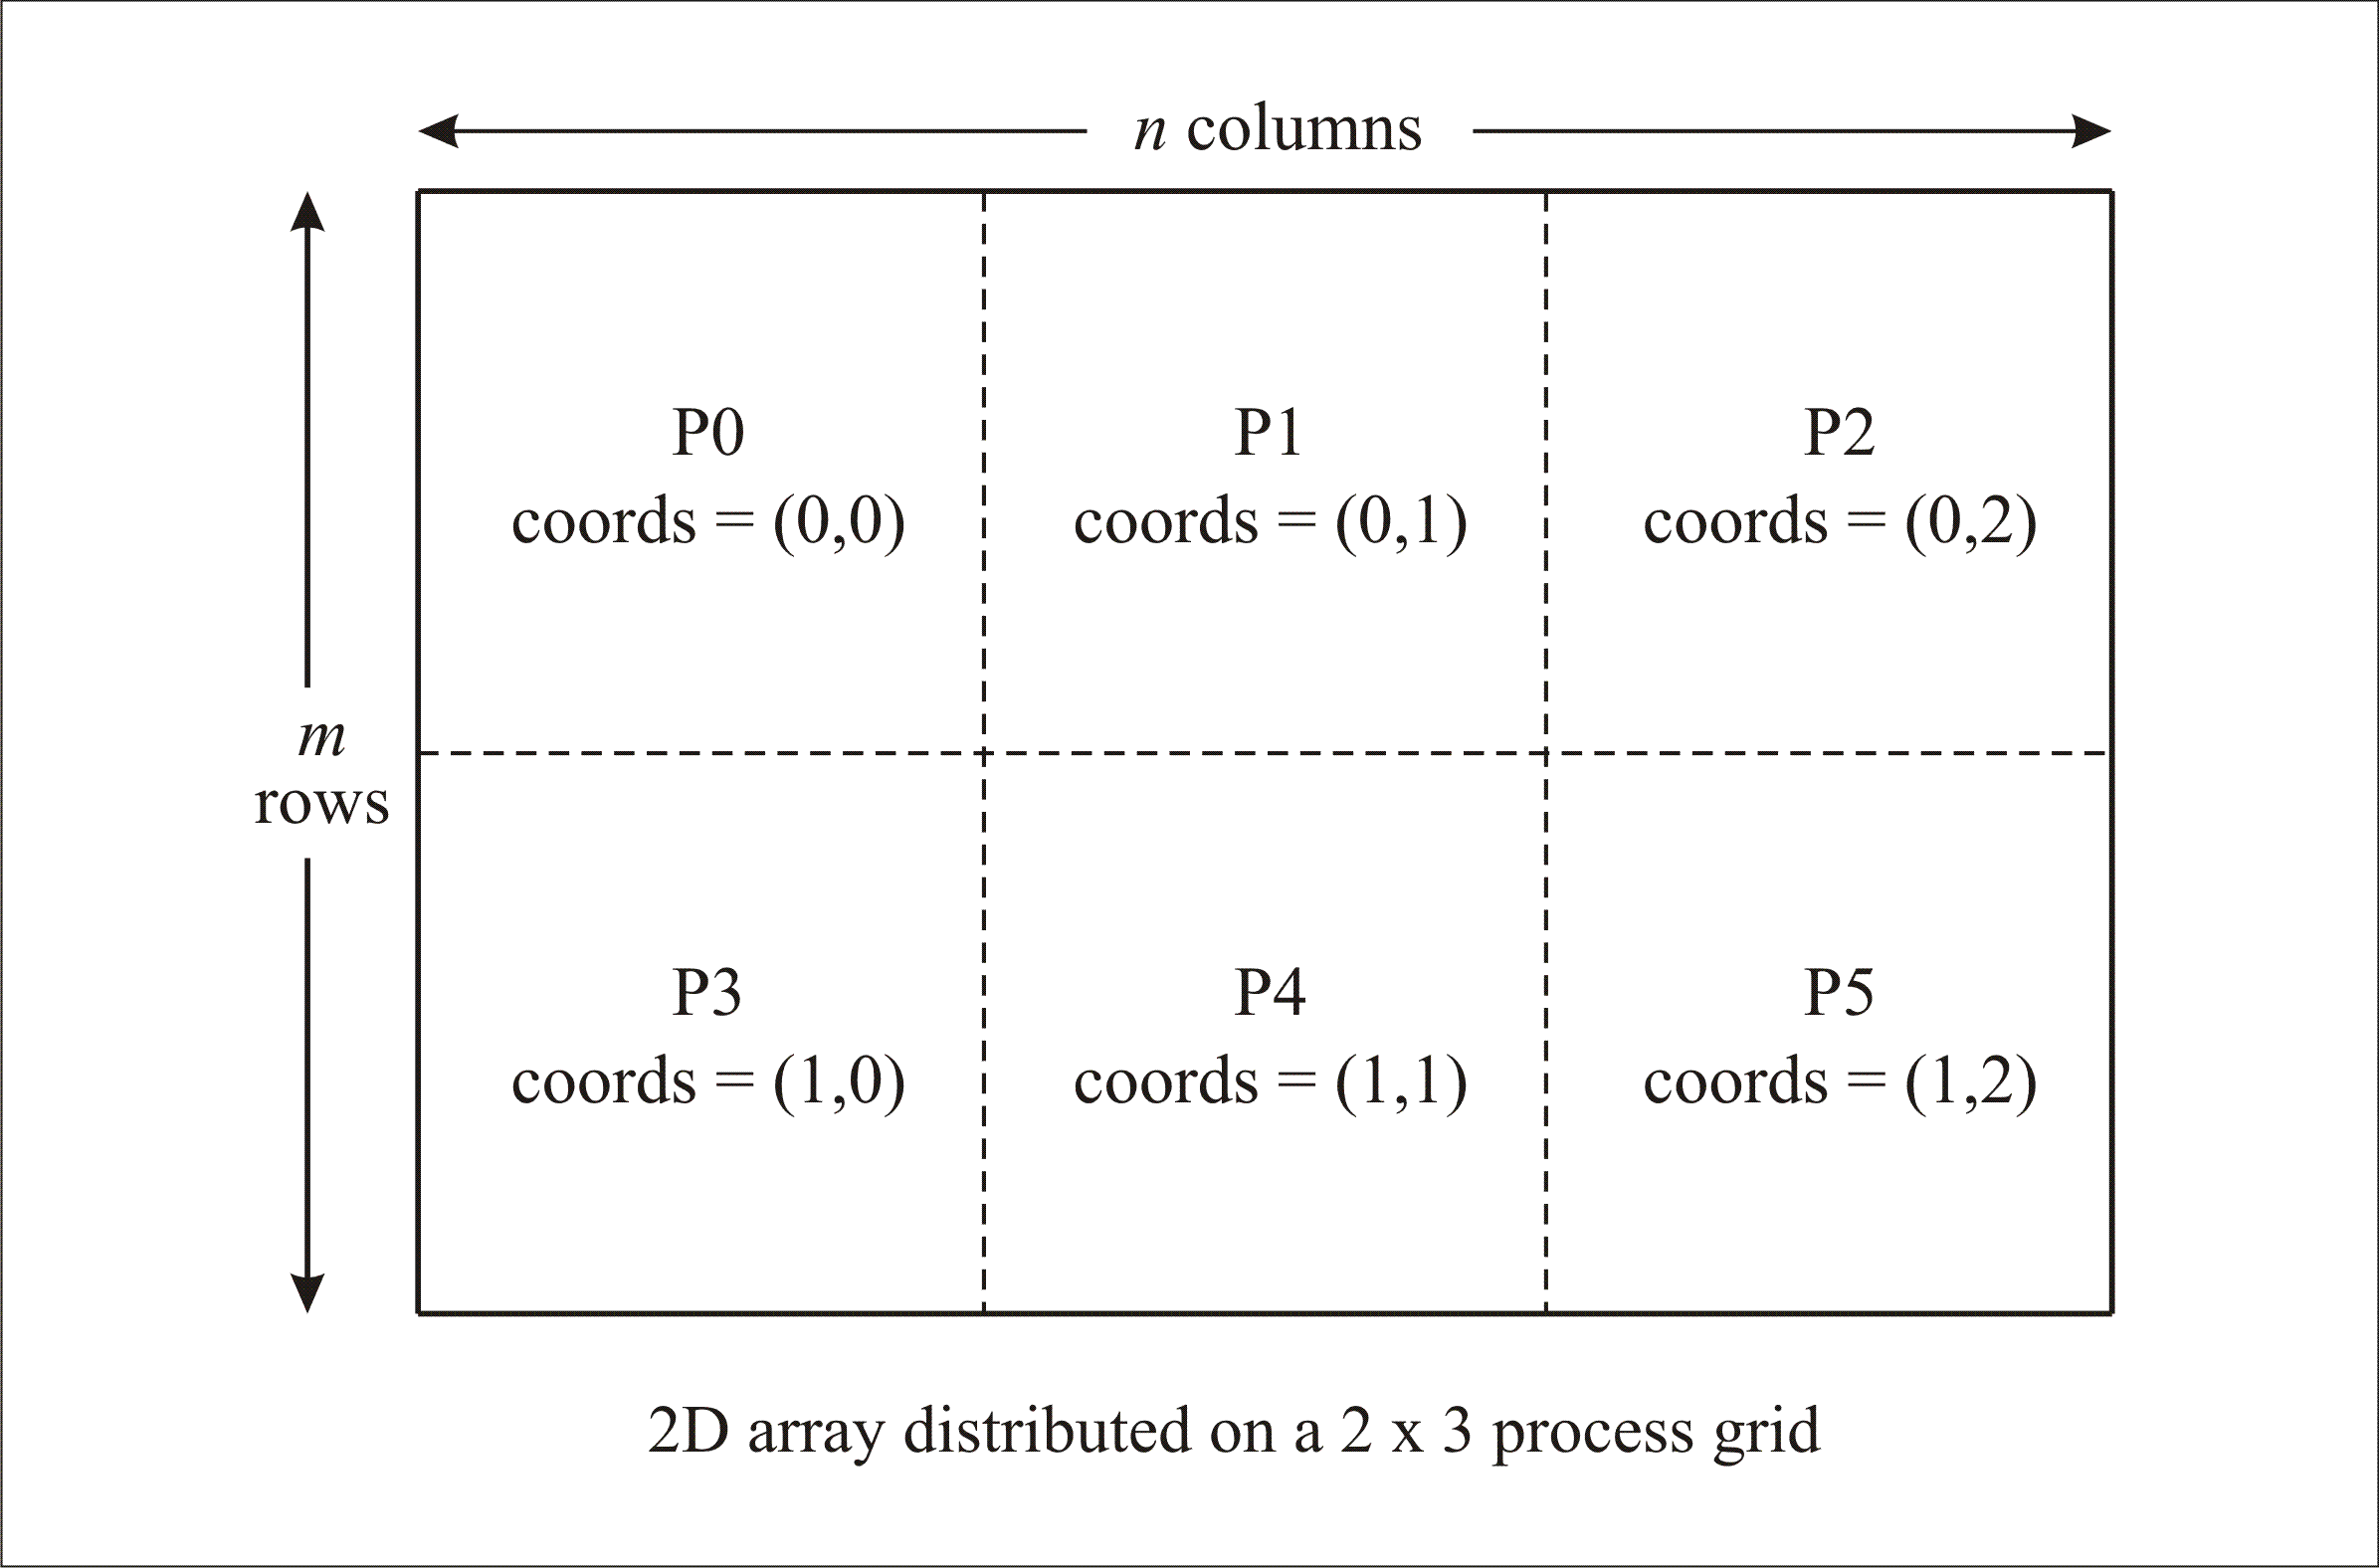
\includegraphics[width=1\textwidth]{slike/darray.png}
  \caption{Подељени низ}
\end{figure}

Осми аргумент функције \texttt{MPI\_Type\_create\_darray} одређује редослед складиштења локалног низа у меморији, као и глобалног низа у фајлу. Девети аргумент је \textit{datatype} који описује ког је типа елемент низа, у овом програму \texttt{MPI\_FLOAT}. Повратна вредност функције је изведени тип података \textit{\&filetype}. После комитовања типа података, нови тип може се користити у постављању погледа(Листинг 2.10). 


\subsection{Неблокирајуће У/И операције и подељене колективне У/И операције}

MPI подржава неблокирајућу верзију независних функција за писање и читање. MPI механизам омогућава ове функције, слично као и неблокирајуће интерпроцесне комуникације. Неблокирајуће функције почињу са 
\texttt{MPI\_File\_ixxx}, нпр.  \texttt{MPI\_File\_iread} и \texttt{MPI\_File\_iwrite\_at}. Неблокирајуће функције враћају \texttt{MPI\_Request} објекат. Могу се користити уобичајене MPI\_Test и MPI\_Wait операције. Користећи ове функције, може доћи до преклапања улазно/излазних операција са осталим комуникацијама у програму. Ова преклапања зависе од квалитета имплементације. За колективне операције, MPI подржава 
ограничен облик неблокирајућих операција, које се називају подељеним колективним У/И операцијама. Да би се користиле подељене колективне функције, корисник мора позвати \zn почетак" функције (\texttt{MPI\_File\_read\_all\_begin}) да би се покренула колективна У/И, као и "крај" функције (\texttt{MPI\_File\_read\_all\_end}) да би се она завршила. Ограничење је да корисник у исто време може имати само једну подељену колективну операцију над једним фајлом. Подељене колективне функције не враћају \texttt{MPI\_Request} објекат.

\subsection{Подељени фајл показивачи}

Постоји три начина да се одреди локација у фајлу са које је потребно прочитати или уписати податке: појединачни фајл показивачи, експлицитна одступања и подељени фајл показивачи.
\textbf{Подељени фајл показивач} је фајл показивач чија вредност је подељена између процеса који се налазе у комуникатору функције \texttt{MPI\_File\_open}. MPI пружа функције \texttt{MPI\_File\_read\_shared} и \texttt{MPI\_File\_write\_shared} које читају/уписују податке са почетком у тренутној локацији подељеног фајл показивача. После позивања ових функција, подељени фајл показивач биће освежен новом количином података који су уписани или прочитани. Следећи позив ових функција ће радити са освеженим подељеним фајл показивачем. Процес може експлицитно померити показивач у \textit{etypes} јединици помоћу функције \texttt{MPI\_File\_seek\_shared}. MPI захтева да сви процеси имају исти фајл поглед када користе подељене фајл показиваче. За остала два начина могу се користити различити фајл погледи. 

